\documentclass[conference]{IEEEtran}
\IEEEoverridecommandlockouts

\usepackage[utf8]{inputenc}
\usepackage[T1]{fontenc}
\usepackage[brazilian]{babel}
\usepackage{amsmath,amssymb,amsfonts}
\usepackage{graphicx}
\usepackage{booktabs}
\usepackage{multirow}
\usepackage{url}
\usepackage[hidelinks]{hyperref}
\usepackage{cite}
\usepackage{balance}

\graphicspath{{../results/summary/}}

\begin{document}
\balance

\title{Impacto do Nível de Abstração em GPU no Treinamento e Inferência de Modelos Transformer: Uma Análise Empírica entre PyTorch, Triton e CUDA C++}

\author{\IEEEauthorblockN{Caleb Martim de Oliveira}
\IEEEauthorblockA{\textit{Departamento de Ciência da Computação (CIC)} \\
\textit{Universidade de Brasília (UnB)}\\
Brasília, Brasil \\
\url{https://github.com/CalebMartim/gpt-implementations}}
}

\renewcommand{\IEEEkeywordsname}{Palavras-chave}
\maketitle

\begin{abstract}
O custo de treinar e servir modelos Transformer depende tanto da aritmética executada quanto da forma como o código chega à GPU, mas a escolha entre frameworks de alto nível e kernels escritos à mão raramente se apoia em medições controladas. Este trabalho compara três implementações matematicamente equivalentes de um Transformer decodificador com 10.788.929 parâmetros: PyTorch \textit{eager}, PyTorch com kernels Triton (atenção fundida no estilo FlashAttention, LayerNorm e entropia cruzada) e um motor nativo em CUDA C++ com cuBLAS. As três partem dos mesmos pesos e lotes (semente 998244353), operam em FP32 estrito e foram medidas em uma NVIDIA A100-SXM4-40GB, com perda inicial idêntica (4,175149) e perda final de treino próxima de 0,192. Cada nível de abstração vence em um regime distinto. Na geração com lote 1, o CUDA C++ atinge 2,00~ms por token, contra 3,90~ms no PyTorch e 6,49~ms no Triton. Com lote 64, o Triton alcança 2.716,9~tokens/s, 14,4\% acima do PyTorch, e reduz o pico de memória de treino em 434,9~MB. No treinamento, o PyTorch, com 120 linhas de código no núcleo, iguala o Triton (704 linhas) e supera o CUDA C++ (1.032 linhas) em vazão.
\end{abstract}

\begin{IEEEkeywords}
Transformers, Programação em GPU, CUDA, OpenAI Triton, PyTorch, Desempenho Computacional, Complexidade de Código (SLOC).
\end{IEEEkeywords}

% ======================================================================
\section{Introdução}
\label{sec:introducao}

Modelos de linguagem baseados na arquitetura Transformer~\cite{vaswani2017attention,radford2019language} tornaram o desempenho de GPUs um fator direto de custo em pesquisa e em produção. O treinamento consome milhares de horas de acelerador, e a inferência autoregressiva impõe restrições de latência por token que afetam diretamente a experiência de uso. Por isso, a pergunta sobre como escrever o código que executa esses modelos tem consequências mensuráveis em tempo, energia e memória.

A forma dominante de programar esses modelos é o PyTorch em modo \textit{eager}~\cite{paszke2019pytorch}, que oferece alta produtividade, mas executa cada operador como um kernel isolado despachado pelo interpretador Python. Essa decomposição tem dois custos conhecidos. Primeiro, cada operador elementar lê e escreve seus tensores na memória global (HBM), de modo que cadeias de operações leves ficam limitadas pela largura de banda e não pela capacidade aritmética~\cite{ivanov2021data}. Segundo, cada lançamento passa pelo interpretador e pelo despachante do framework, o que gera um custo fixo na CPU que domina quando o volume de trabalho por kernel é pequeno. As alternativas são descer para uma linguagem de blocos como o Triton~\cite{tillet2019triton}, que permite fundir operadores em memória compartilhada (SRAM) sem abandonar o Python, ou escrever o motor inteiro em CUDA C++, como no projeto llm.c~\cite{karpathy2024llmc}, eliminando o interpretador.

O ganho de cada alternativa raramente é quantificado em conjunto com o seu custo de engenharia. Comparações publicadas costumam isolar um único kernel, por exemplo a atenção~\cite{dao2022flashattention}, ou usam modelos e precisões diferentes entre implementações, o que impede atribuir a diferença de desempenho ao nível de abstração. Este trabalho responde, sob condições controladas, à seguinte questão de pesquisa: \textit{em que medida o nível de abstração de programação em GPU (PyTorch eager, Triton e CUDA C++) afeta o tempo de execução, a vazão de treinamento e de inferência, o consumo de memória e a complexidade de implementação de um modelo Transformer?}

Para isolar esse fator, implementamos o mesmo modelo três vezes, com pesos iniciais, sequência de lotes e precisão numérica idênticos, e verificamos a equivalência matemática antes de qualquer medição de tempo. As contribuições do trabalho são três:
\begin{itemize}
\item um protocolo experimental reprodutível, com verificação de paridade numérica nos passos 0 e 1 e treinamento em FP32 estrito, que permite atribuir as diferenças de desempenho apenas à implementação;
\item a caracterização de uma especialização por regime de carga: o CUDA C++ vence em latência com lote 1, o Triton vence em vazão com lote 64 e em memória, e o PyTorch empata ou vence no treinamento, cada resultado explicado por um mecanismo de hardware específico;
\item uma auditoria de linhas de código (SLOC) que posiciona as três implementações em uma fronteira de Pareto entre desempenho e esforço de engenharia.
\end{itemize}

A Seção~\ref{sec:fundamentacao} apresenta os fundamentos, a Seção~\ref{sec:metodologia} descreve o desenho experimental, a Seção~\ref{sec:resultados} interpreta os resultados e a Seção~\ref{sec:conclusao} conclui.

% ======================================================================
\section{Fundamentação Teórica}
\label{sec:fundamentacao}

\subsection{Transformer Decodificador com Atenção Causal}

O modelo estudado é um Transformer somente-decodificador no estilo GPT~\cite{radford2019language}, que prevê o próximo token a partir dos anteriores. A entrada de $T$ tokens é convertida na soma de \textit{embeddings} de token e de posição, de dimensão $C$, e atravessa $L$ blocos idênticos. Cada bloco aplica LayerNorm antes de cada subcamada (arranjo \textit{Pre-LN}~\cite{xiong2020layer}), seguida de atenção multi-cabeça causal e de uma rede \textit{feed-forward} com expansão $4C$ e ativação ReLU, ambas com conexão residual.

A atenção concentra o custo de memória que motiva este estudo. Para cada cabeça, o bloco calcula
\begin{equation}
\text{Atenção}(Q,K,V)=\mathrm{softmax}\!\left(\frac{QK^\top}{\sqrt{d_k}}+M\right)V,
\label{eq:attn}
\end{equation}
em que $M$ é a máscara causal que atribui $-\infty$ às posições futuras e $d_k=C/H$ é a dimensão por cabeça. A matriz intermediária $QK^\top$ tem formato $(B,H,T,T)$ para um lote de $B$ sequências e $H$ cabeças. Como seu tamanho cresce com $T^2$, ela supera rapidamente o volume das ativações de formato $(B,T,C)$: na configuração usada aqui, cada uma dessas matrizes ocupa 96~MB em FP32 por camada.

\subsection{Hierarquia de Memória da GPU}

Uma GPU moderna combina uma memória global grande e relativamente lenta com memórias pequenas e rápidas dentro de cada multiprocessador. A NVIDIA A100-SXM4-40GB oferece 40~GB de HBM2 com largura de banda nominal de 1.555~GB/s e, em cada um dos 108 multiprocessadores (SMs), até 164~KB de memória compartilhada (SRAM) configurável~\cite{nvidia2020a100}. Sua capacidade de pico em FP32 sem Tensor Cores é de 19,5~TFLOP/s. O modelo \textit{roofline}~\cite{williams2009roofline} explica a consequência: um kernel que realiza poucas operações por byte transferido, como uma soma elementar ou uma softmax, fica limitado pela HBM, enquanto multiplicações de matrizes densas (GEMMs) ficam limitadas pela aritmética.

A fusão de operadores reduz o tráfego na HBM ao manter resultados intermediários na SRAM. O FlashAttention~\cite{dao2022flashattention,dao2024flashattention2} aplica essa ideia à Equação~\eqref{eq:attn}: processa $Q$, $K$ e $V$ em blocos, calcula a softmax de forma incremental com o normalizador \textit{online}~\cite{milakov2018online} e nunca escreve a matriz $(B,H,T,T)$ na memória global. No passo de retropropagação, a matriz é recalculada bloco a bloco a partir de $Q$, $K$ e de uma estatística de normalização por linha. O método troca, portanto, tráfego de memória por operações aritméticas adicionais.

Um segundo custo, independente da GPU, é o despacho feito pela CPU. Cada lançamento de kernel exige que o processo hospedeiro prepare argumentos e enfileire o comando, e em frameworks Python esse caminho inclui o interpretador e o despachante de operadores. Quando cada kernel processa pouco dado, como na geração de um único token, a GPU termina o trabalho antes de receber o próximo comando e passa a esperar pela CPU.

\subsection{Paradigmas de Programação em GPU}

Os três paradigmas comparados diferem na granularidade em que o programador controla a execução. No PyTorch \textit{eager}~\cite{paszke2019pytorch}, o modelo é escrito como uma sequência de operadores de tensor, cada um mapeado para um kernel pré-compilado, e o motor \textit{autograd} constrói dinamicamente o grafo de retropropagação. O programador não controla a fusão nem a disposição dos dados na memória rápida.

O Triton~\cite{tillet2019triton} é uma linguagem embutida em Python na qual o programador descreve o trabalho de um bloco de threads sobre \textit{tiles} de dados, e o compilador gera o código de GPU e gerencia a SRAM e a sincronização entre threads. Esse nível permite escrever kernels fundidos como o FlashAttention em algumas centenas de linhas. Os kernels são integrados ao PyTorch por meio de \texttt{torch.autograd.Function}, de modo que o restante do modelo continua em Python.

No CUDA C++, o programador escreve cada kernel no nível de thread, controla explicitamente a memória compartilhada e as primitivas de \textit{warp}, e invoca bibliotecas como o cuBLAS para as GEMMs. Um motor inteiramente nativo, como o llm.c~\cite{karpathy2024llmc}, elimina o interpretador do laço de execução, mas exige implementar manualmente a retropropagação de cada operador e o otimizador.

% ======================================================================
\section{Metodologia}
\label{sec:metodologia}

\subsection{Desenho Experimental e Variáveis}

O estudo segue um desenho experimental com um único fator, o nível de abstração, avaliado em três níveis: \texttt{01\_pytorch}, \texttt{02\_triton} e \texttt{03\_cuda\_cpp}. As variáveis dependentes são: (i) o tempo de parede de 5.000 passos de treinamento e a vazão correspondente, $5000 \times 64 \times 256 / t_{\mathrm{treino}}$ tokens/s; (ii) o tempo de geração autoregressiva de 1.000 tokens com lote $B=1$, reportado como latência por token, e com lote $B=64$, reportado como vazão $B \times 1000 / t_{\mathrm{inf}}$; (iii) o pico de memória de vídeo (VRAM); e (iv) o número de linhas de código-fonte (SLOC). As curvas de perda de treino e validação servem como variável de controle da equivalência numérica.

A contagem de SLOC é feita por um script auditável (\texttt{common/count\_sloc.py}) que exclui linhas em branco, comentários e \textit{docstrings}. As linhas são separadas em núcleo, que reúne a definição do modelo, o passo direto, a retropropagação, os kernels e o otimizador, e em \textit{harness}, que reúne carregamento de dados, cronometragem e exportação dos resultados. No arquivo \texttt{.cu}, a fronteira é marcada por um comentário delimitador explícito.

\subsection{Controle de Variáveis e Paridade Numérica}

Todas as execuções usaram a mesma GPU NVIDIA A100-SXM4-40GB no Google Colab Pro, o mesmo modelo e os mesmos hiperparâmetros, resumidos na Tabela~\ref{tab:hiperparametros}. O corpus é o TinyShakespeare, com 1.115.394 caracteres, tokenizado por caractere em um vocabulário de 65 símbolos e dividido em 90\% para treino e 10\% para validação. O otimizador é o AdamW~\cite{loshchilov2019decoupled} e o \textit{dropout} é nulo, o que remove a única fonte de aleatoriedade durante o treinamento.

\begin{table}[t]
\centering
\caption{Hiperparâmetros invariantes nas três implementações.}
\label{tab:hiperparametros}
\begin{tabular}{@{}llr@{}}
\toprule
Hiperparâmetro & Símbolo & Valor \\
\midrule
Lote de treino & $B$ & 64 \\
Contexto & $T$ & 256 \\
Dimensão de \textit{embedding} & $C$ & 384 \\
Cabeças de atenção & $H$ & 6 ($d_k=64$) \\
Camadas & $L$ & 6 \\
Parâmetros treináveis & $|\theta|$ & 10.788.929 \\
Passos de treino & -- & 5.000 \\
AdamW & $\eta,\ \beta_1,\ \beta_2,\ \lambda$ & $3{\cdot}10^{-4}$, 0,9, 0,999, 0,01 \\
Semente global & -- & 998244353 \\
Precisão & -- & FP32 (sem TF32) \\
\bottomrule
\end{tabular}
\end{table}

Para eliminar diferenças de inicialização e de amostragem, um script comum gera, com a semente 998244353, os pesos iniciais $\theta_0$ (distribuição $\mathcal{N}(0;\,0{,}02)$) e a sequência completa de lotes $(X_t, Y_t)$ para $t \in [0, 4999]$, e grava ambos em disco. As três implementações carregam esses mesmos artefatos. A precisão é fixada em FP32 IEEE~754: no PyTorch e no Triton, \texttt{allow\_tf32} é desativado tanto nas bibliotecas quanto nas chamadas \texttt{tl.dot}, e no motor nativo o cuBLAS opera em \texttt{CUBLAS\_PEDANTIC\_MATH}. Sem essa restrição, os Tensor Cores da A100 usariam TF32, com mantissa de 10 bits, e as implementações divergiriam por arredondamento e não por diferença de código.

Antes de cada medição, um portão de sanidade compara a perda no passo 0 e, após uma atualização do AdamW, a perda no passo 1 com valores de referência. A execução é abortada se qualquer diferença ultrapassar $10^{-4}$. Esse portão garante que as medições de tempo comparam programas que calculam a mesma função.

\subsection{Implementações}

A implementação \texttt{01\_pytorch} (120 SLOC no núcleo) é a referência e segue o código de Karpathy~\cite{karpathy2023nanogpt}. A atenção é escrita com operadores explícitos (\texttt{q @ k.transpose}, multiplicação pela escala, \texttt{masked\_fill} e \texttt{softmax}), e a retropropagação fica a cargo do \textit{autograd}. Cada um desses operadores materializa um tensor $(B,H,T,T)$ na HBM.

A implementação \texttt{02\_triton} (704 SLOC no núcleo) mantém as camadas lineares do PyTorch e substitui os operadores limitados por memória por seis kernels \texttt{@triton.jit}. São eles: atenção causal fundida nos passos direto e reverso, no estilo FlashAttention, com blocos de $32 \times 32$ e softmax \textit{online}; LayerNorm direta com redução de média e variância em um único passe; dois kernels de retropropagação da LayerNorm, um para $dX$ e outro para a redução de $d\gamma$ e $d\beta$; e um kernel que calcula a entropia cruzada e o gradiente dos \textit{logits} em uma única leitura. O passo direto da atenção grava apenas a saída e o vetor de log-soma-exponencial por linha, e o passo reverso recalcula os blocos de $QK^\top$.

A implementação \texttt{03\_cuda\_cpp} (1.032 SLOC no núcleo) é um executável autônomo compilado com \texttt{nvcc -O3} e ligado ao cuBLAS. As projeções lineares usam \texttt{cublasSgemm} e os produtos da atenção usam \texttt{cublasSgemmStridedBatched}. Os demais operadores são 17 kernels \texttt{\_\_global\_\_} escritos à mão, que cobrem \textit{embedding}, LayerNorm, softmax causal com escala e máscara fundidas, ReLU, soma residual, transposições de cabeças, entropia cruzada, AdamW e \textit{argmax}, com reduções feitas por \texttt{\_\_shfl\_xor\_sync}. Todas as ativações e gradientes residem em uma arena estática alocada uma única vez no início, e nenhum código Python executa durante o treinamento ou a geração. Esta versão não funde a atenção: as matrizes de escores e de probabilidades são materializadas e armazenadas por camada.

\subsection{Protocolo de Medição}

Cada implementação executa 50 passos de aquecimento, recarrega $\theta_0$, reinicia o otimizador e então mede os 5.000 passos de treinamento. As avaliações de perda, feitas a cada 500 passos com 50 lotes por partição, ficam fora do cronômetro, e todas as fronteiras de medição são precedidas de sincronização com o dispositivo. A geração é gulosa (\textit{argmax}), parte de um token inicial e não usa \textit{cache} de chaves e valores (KV-\textit{cache}). Assim, cada novo token exige um passo direto completo sobre uma janela de até 256 tokens, nas três implementações. Cada configuração foi executada uma vez.

A memória é medida por mecanismos diferentes, o que restringe a comparação. No PyTorch e no Triton, \texttt{torch.cuda.max\_memory\_allocated} reporta o pico de tensores do alocador do PyTorch durante o treinamento, sem incluir o contexto CUDA nem o \textit{cache} do alocador. No CUDA C++, \texttt{cudaMemGetInfo} reporta a memória ocupada em toda a placa, incluindo o contexto do driver e o espaço de trabalho do cuBLAS. Os valores são expressos em MB de $2^{20}$ bytes.

% ======================================================================
\section{Resultados}
\label{sec:resultados}

A Tabela~\ref{tab:resultados} reúne as métricas das três implementações, e a Fig.~\ref{fig:throughput} compara as vazões nos três regimes de carga. A leitura conjunta mostra que nenhuma implementação domina todas as métricas: cada uma vence no regime em que o seu nível de abstração remove o gargalo dominante.

\begin{table*}[t]
\centering
\caption{Resultados na NVIDIA A100-SXM4-40GB (FP32 estrito, execução única). Setas indicam a direção desejável; o melhor valor de cada coluna está em negrito. A VRAM do CUDA C++ é medida pela ocupação global da placa e não é diretamente comparável (Seção~\ref{sec:vram}).}
\label{tab:resultados}
\begin{tabular}{@{}lrrrrrrr@{}}
\toprule
& \multicolumn{1}{c}{Código} & \multicolumn{2}{c}{Treinamento} & \multicolumn{2}{c}{Inferência $B=1$} & \multicolumn{1}{c}{Inferência $B=64$} & \multicolumn{1}{c}{Memória} \\
\cmidrule(lr){2-2}\cmidrule(lr){3-4}\cmidrule(lr){5-6}\cmidrule(lr){7-7}\cmidrule(l){8-8}
Implementação & SLOC núcleo $\downarrow$ & Tempo (s) $\downarrow$ & tokens/s $\uparrow$ & ms/token $\downarrow$ & tokens/s $\uparrow$ & tokens/s $\uparrow$ & VRAM (MB) $\downarrow$ \\
\midrule
PyTorch \textit{eager} & \textbf{120} & \textbf{473,00} & \textbf{173.193,7} & 3,90 & 256,4 & 2.375,3 & 2.675,3 \\
PyTorch + Triton & 704 & 474,73 & 172.562,6 & 6,49 & 154,0 & \textbf{2.716,9} & \textbf{2.240,4} \\
CUDA C++ + cuBLAS & 1.032 & 493,39 & 166.033,4 & \textbf{2,00} & \textbf{500,0} & 2.538,5 & 5.611,9$^{*}$ \\
\bottomrule
\multicolumn{8}{@{}l}{\footnotesize $^{*}$Medido com \texttt{cudaMemGetInfo}; inclui contexto do driver, espaço de trabalho do cuBLAS e a arena estática de ativações.}
\end{tabular}
\end{table*}

\begin{figure*}[t]
\centering
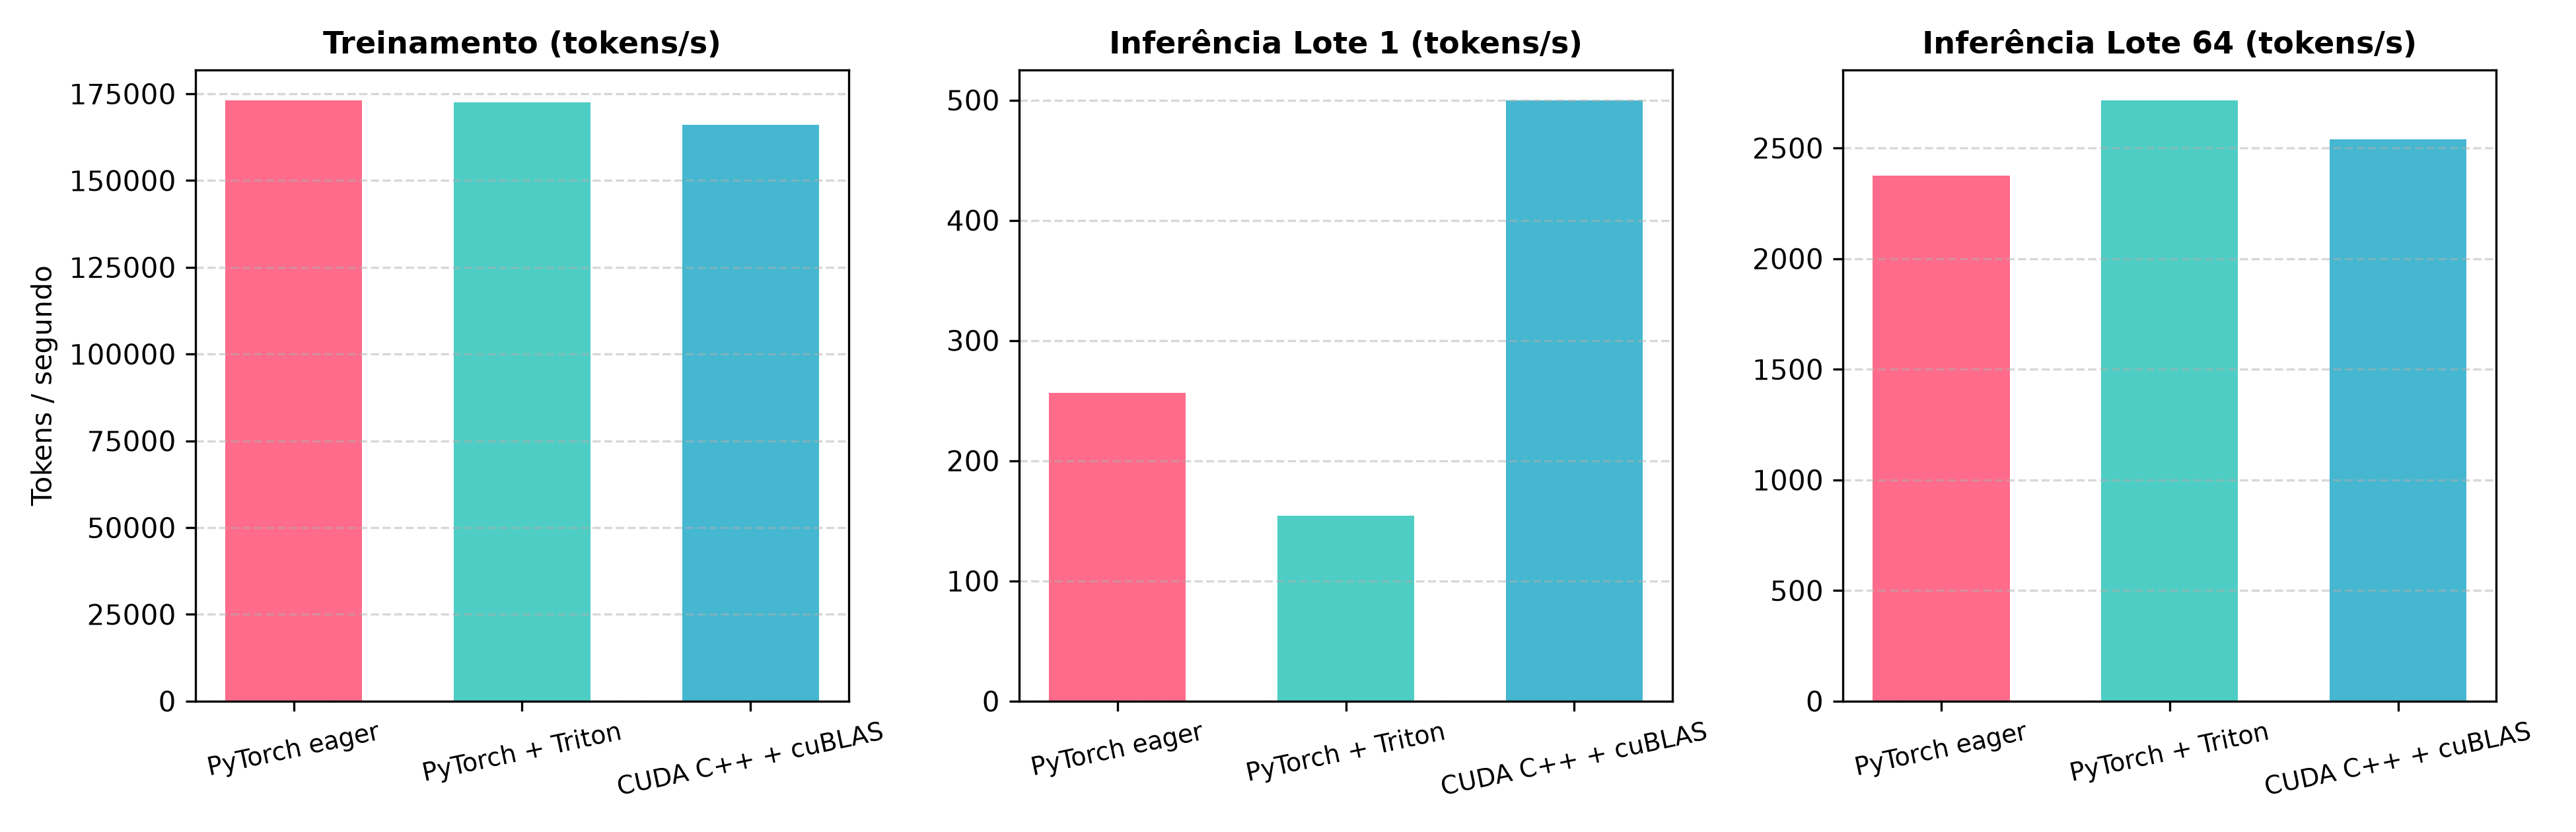
\includegraphics[width=0.9\textwidth]{throughput_comparison.png}
\caption{Vazão em tokens/s no treinamento (esquerda), na geração com lote 1 (centro) e na geração com lote 64 (direita). A ordem das implementações se inverte entre os regimes.}
\label{fig:throughput}
\end{figure*}

\subsection{Paridade Numérica e Convergência}

As três implementações calculam a mesma função de perda a partir do mesmo ponto inicial. A perda no passo 0 é 4,175149 nas três, com diferença nula em relação à referência, e a perda no passo 1, após a primeira atualização do AdamW, difere da referência em $2{,}1 \times 10^{-6}$ (PyTorch), $3{,}1 \times 10^{-6}$ (Triton) e $2{,}6 \times 10^{-6}$ (CUDA C++). Essas diferenças estão duas ordens de grandeza abaixo do limiar de $10^{-4}$ e são compatíveis com a ordem distinta de acumulação em ponto flutuante entre kernels~\cite{goldberg1991floating}.

As trajetórias de otimização permanecem sobrepostas ao longo dos 5.000 passos, como mostra a Fig.~\ref{fig:loss}. A perda de treino final é 0,1919 (PyTorch), 0,1918 (Triton) e 0,1925 (CUDA C++), uma dispersão inferior a 0,4\%. A perda de validação atinge o mínimo próximo de 1,54 no passo 1.000 nas três versões e depois cresce até cerca de 3,6, um sobreajuste esperado para um modelo de 10,8~milhões de parâmetros treinado sem \textit{dropout} sobre cerca de um milhão de caracteres. Esse comportamento não afeta a comparação de desempenho, pois o custo por passo independe do valor da perda, mas explica a dispersão maior da perda de validação final (3,606 a 3,678). Os kernels de \textit{embedding} e de LayerNorm do CUDA C++ e o gradiente $dQ$ da atenção em Triton acumulam por operações atômicas, cuja ordem não é determinística, e as pequenas diferenças resultantes se amplificam no regime de sobreajuste.

\begin{figure}[t]
\centering
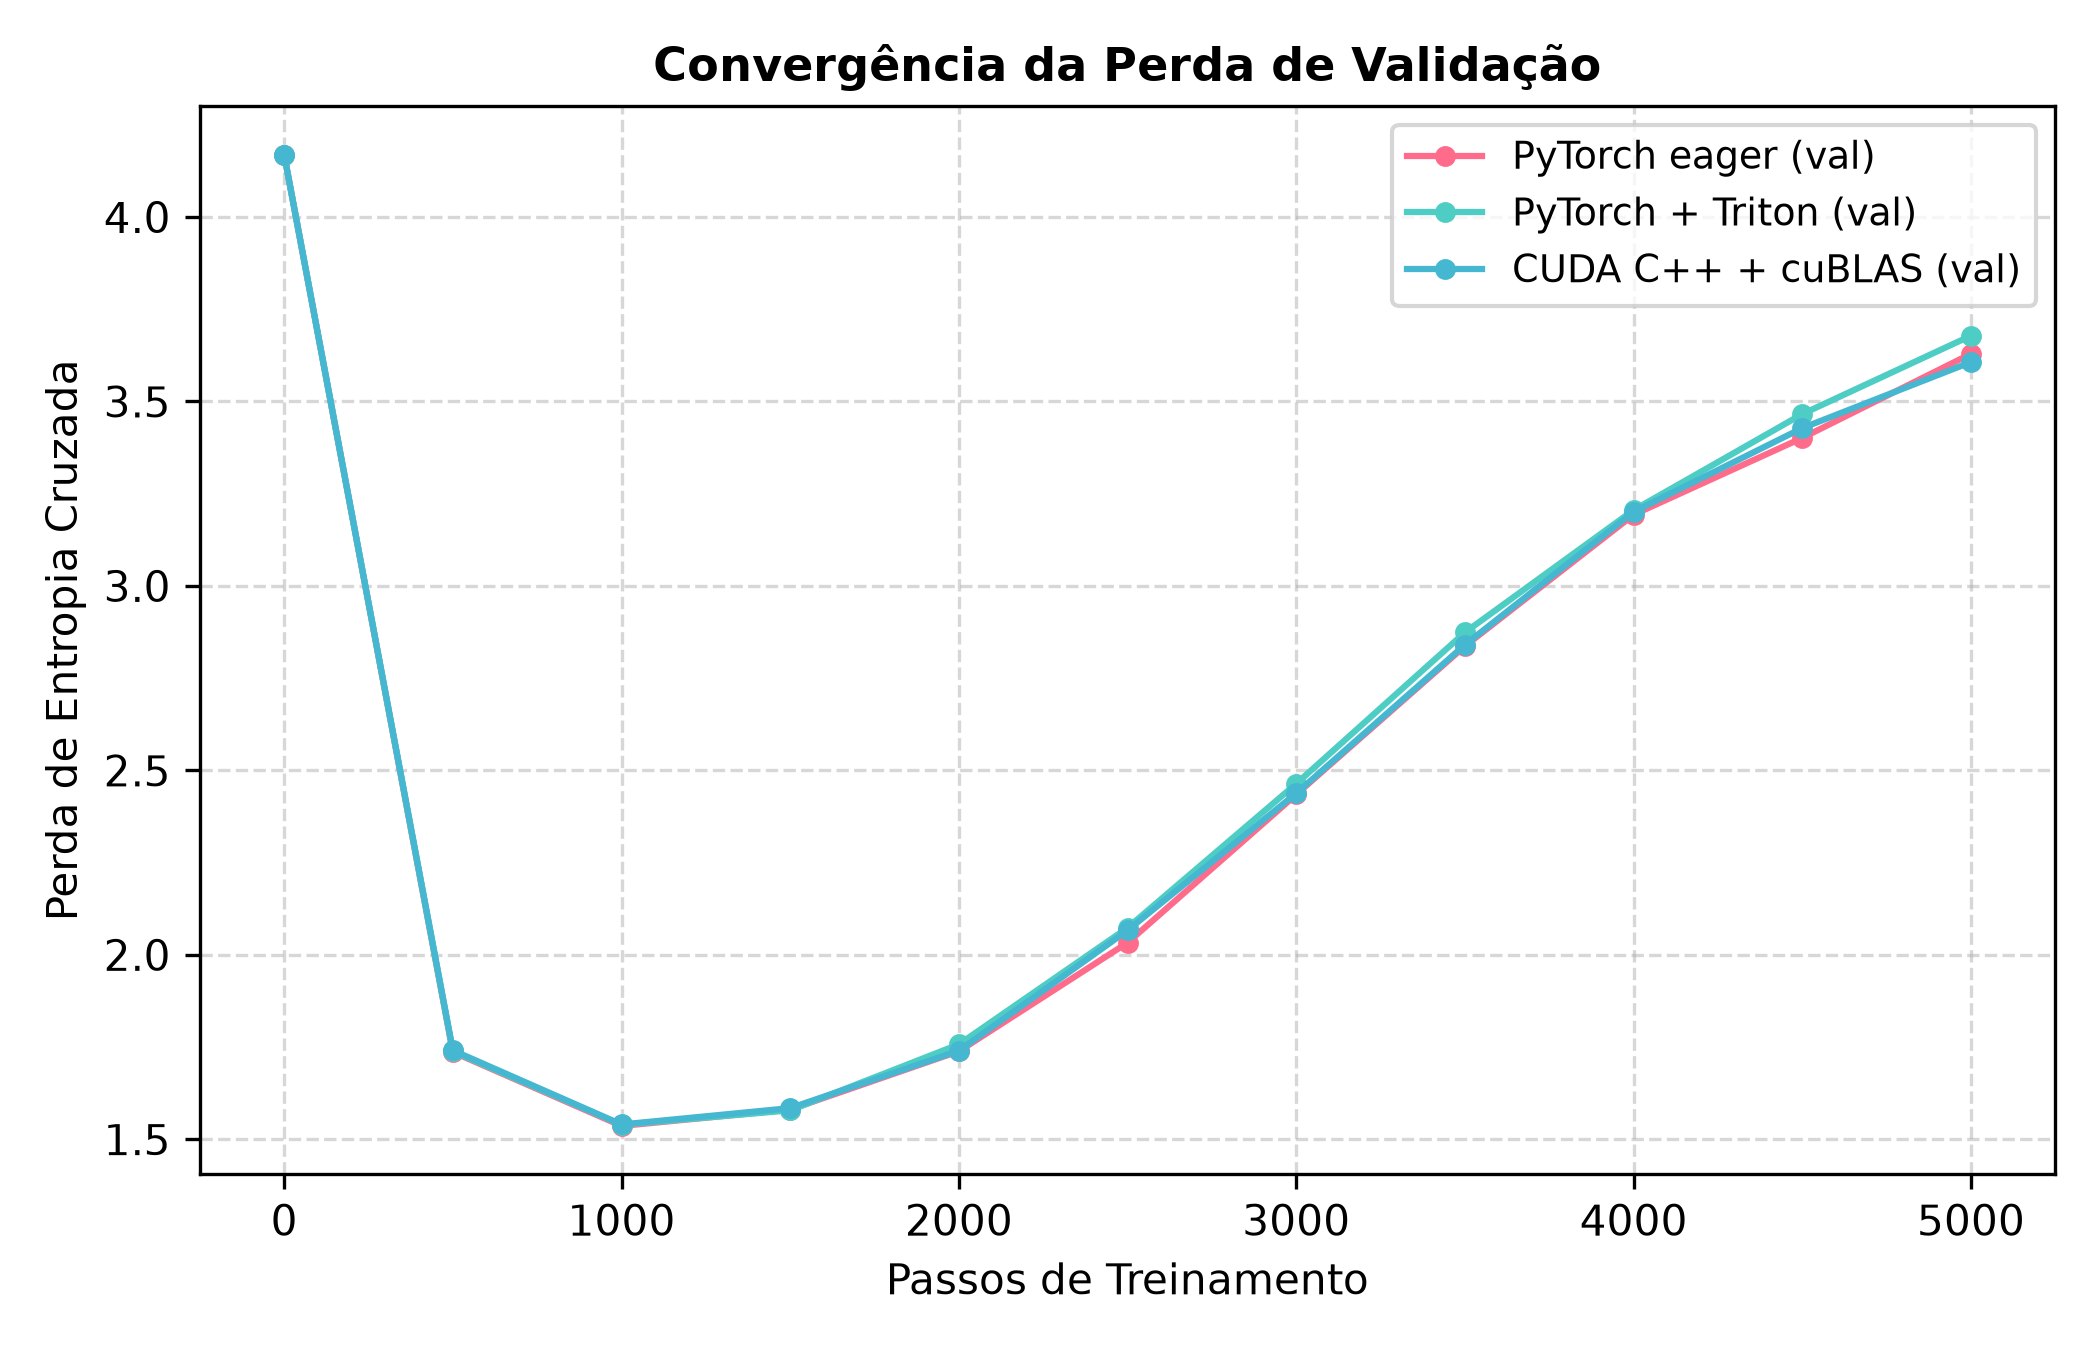
\includegraphics[width=0.92\columnwidth]{loss_convergence.png}
\caption{Perda de validação a cada 500 passos. As três curvas coincidem até o mínimo e divergem apenas no regime de sobreajuste.}
\label{fig:loss}
\end{figure}

\subsection{Treinamento: Domínio das GEMMs em FP32}

No treinamento, as três implementações ficam a menos de 5\% umas das outras. O Triton é 0,36\% mais lento que o PyTorch (474,73~s contra 473,00~s), e o CUDA C++ é 4,1\% mais lento (493,39~s). A proximidade decorre da composição do custo de cada passo. Uma estimativa de primeira ordem, $6|\theta|BT$ operações para as camadas densas mais as duas multiplicações da atenção nos passos direto e reverso, resulta em cerca de 1,18~TFLOP por passo. Com 94,6~ms por passo no PyTorch, isso corresponde a aproximadamente 12,4~TFLOP/s, ou 64\% do pico de 19,5~TFLOP/s da A100 em FP32. O passo de treino é, portanto, limitado pela aritmética das GEMMs, e as três versões executam essas GEMMs no mesmo cuBLAS em FP32.

As otimizações de cada versão atuam sobre a fração restante do tempo e têm efeitos opostos. No Triton, a fusão da atenção remove o tráfego da matriz $(B,H,T,T)$, mas o passo reverso do FlashAttention recalcula $QK^\top$ bloco a bloco, o que acrescenta operações. Em FP32 estrito essas operações não podem usar Tensor Cores, e as cópias contíguas de $Q$, $K$ e $V$ exigidas pelo kernel somam tráfego adicional. O efeito líquido é praticamente nulo. No CUDA C++, a ausência do interpretador não traz ganho, porque um passo de treino com 16.384 tokens mantém a GPU ocupada por tempo suficiente para esconder o despacho. Os kernels escritos à mão, sem a sintonia dos kernels de biblioteca, explicam a perda de 4,1\%.

\subsection{\texorpdfstring{Inferência: Latência com $B=1$ e Vazão com $B=64$}{Inferência: Latência com B=1 e Vazão com B=64}}

Com lote 1, o desempenho é determinado pelo custo de despacho na CPU, e o CUDA C++ vence com folga. A latência é de 2,00~ms por token no motor nativo, 3,90~ms no PyTorch e 6,49~ms no Triton, de modo que o CUDA C++ é 1,95 vezes mais rápido que o PyTorch e 3,25 vezes mais rápido que o Triton. Nesse regime, cada passo direto processa no máximo 256 tokens, e cada matriz de atenção ocupa apenas 1,5~MB, de forma que os kernels terminam em poucos microssegundos e a GPU espera pelo próximo comando. Como as três versões lançam essencialmente a mesma sequência de operações, os 2,00~ms do CUDA C++ servem de referência aproximada para o custo de GPU somado ao lançamento nativo. Atribuímos a diferença de 1,90~ms por token no PyTorch ao interpretador Python e ao despachante de operadores, executados a cada um dos aproximadamente cem kernels de um passo direto.

O Triton é o mais lento com lote 1 porque acrescenta custo justamente no caminho que domina esse regime. Cada camada passa por três chamadas a \texttt{autograd.Function} implementadas em Python. Cada chamada prepara a lista de argumentos do kernel, que no caso da atenção inclui 16 \textit{strides}, consulta o \textit{cache} de especializações do compilador e, na atenção, executa três cópias contíguas adicionais. Esse custo fixo por chamada não depende do tamanho do problema e, por isso, pesa mais quando o problema é pequeno. Sem perfilamento com Nsight, tratamos essa decomposição como a explicação mais consistente com os dados e não como uma medição direta.

Com lote 64, a ordem se inverte: o Triton atinge 2.716,9~tokens/s, 14,4\% acima do PyTorch (2.375,3) e 7,0\% acima do CUDA C++ (2.538,5). Cada passo direto passa a processar até $64 \times 256$ tokens, o custo de despacho fica amortizado e o tráfego da matriz de atenção na HBM se torna relevante. A diferença entre as implementações acompanha o número de vezes que cada uma lê e escreve a matriz $(B,H,T,T)$. O PyTorch faz cinco passagens por camada: escreve os escores e depois lê e reescreve a matriz na escala, na máscara e na softmax, antes da leitura final pelo produto com $V$. Ao todo, são cerca de 768~MB de tráfego por camada no contexto máximo. O CUDA C++ funde escala, máscara e softmax em um kernel e reduz esse tráfego à metade, enquanto o Triton não o realiza.

Uma estimativa de primeira ordem confirma que esse mecanismo explica a maior parte das diferenças medidas. Ponderando o comprimento médio da janela ao longo dos 1.000 passos de geração e usando a largura de banda nominal de 1.555~GB/s, o tráfego extra prevê cerca de 2,6~ms por passo para o PyTorch e 1,3~ms para o CUDA C++ em relação ao Triton. As diferenças medidas são 3,4~ms e 1,7~ms por passo. A razão entre as duas diferenças medidas, 0,49, coincide com a razão de 0,5 prevista pela contagem de passagens. O excedente absoluto é compatível com uma largura de banda efetiva inferior à nominal e com a leitura da máscara, que a estimativa não inclui.

\subsection{Consumo de Memória}
\label{sec:vram}

Entre as duas implementações medidas pelo mesmo alocador, o Triton reduz o pico de memória de treino em 434,9~MB, de 2.675,3~MB para 2.240,4~MB, uma redução de 16,3\%. A origem é a mesma da subseção anterior. No PyTorch, o \textit{autograd} guarda a matriz de probabilidades $(B,H,T,T)$ de cada camada para a retropropagação, o que soma $6 \times 96 = 576$~MB. O kernel fundido do Triton guarda apenas a saída e uma estatística por linha, de tamanho $(B,H,T)$. A redução medida é menor que 576~MB porque o Triton guarda as cópias contíguas de $Q$, $K$ e $V$, que no PyTorch são apenas visões do tensor de projeção.

O valor de 5.611,9~MB do CUDA C++ não deve ser comparado diretamente com os anteriores, porque \texttt{cudaMemGetInfo} reporta a ocupação de toda a placa. Somando os tamanhos alocados pelo próprio código, a arena estática ocupa cerca de 5,2~GB. Esse total inclui, por camada, as matrizes de escores e de probabilidades, além de gradientes de atenção, ativações pré e pós-ReLU separadas e estados do AdamW. Os cerca de 0,45~GB restantes são compatíveis com o contexto do driver e o espaço de trabalho do cuBLAS na A100. O consumo maior reflete uma escolha de projeto da versão nativa, que prioriza endereços fixos e simplicidade de retropropagação sobre o reaproveitamento de memória, e não uma propriedade do nível de abstração.

\subsection{Fronteira de Pareto entre SLOC e Desempenho}

A auditoria de código mostra que descer de nível de abstração multiplica o esforço de implementação, como detalha a Tabela~\ref{tab:sloc}. O núcleo do Triton tem 5,9 vezes mais linhas que o do PyTorch, e o do CUDA C++ tem 8,6 vezes mais. O crescimento vem de trabalho que o framework fazia implicitamente: os kernels Triton somam 580 linhas, e o motor nativo precisa implementar a retropropagação de cada operador, o otimizador e a gestão de memória.

\begin{table}[t]
\centering
\caption{Linhas de código-fonte (SLOC) por implementação, sem comentários e linhas em branco.}
\label{tab:sloc}
\begin{tabular}{@{}lrrr@{}}
\toprule
Implementação & Núcleo & \textit{Harness} & Total \\
\midrule
PyTorch \textit{eager} & 120 & 307 & 427 \\
PyTorch + Triton & 704 & 308 & 1.012 \\
CUDA C++ + cuBLAS & 1.032 & 369 & 1.401 \\
\bottomrule
\end{tabular}
\end{table}

Para o treinamento, o PyTorch domina as outras duas versões no sentido de Pareto, pois tem ao mesmo tempo o menor código e a maior vazão, como mostra a Fig.~\ref{fig:pareto}. As 584 linhas adicionais do Triton não trazem ganho de vazão de treino, e as 912 linhas adicionais do CUDA C++ resultam em uma perda de 4,1\%. A fronteira muda nos outros regimes. Na geração com lote 64 e no consumo de memória, as 584 linhas do Triton compram 14,4\% de vazão e 16,3\% de redução de VRAM. Na geração com lote 1, as 912 linhas do CUDA C++ compram uma latência 1,95 vezes menor. A escolha do nível de abstração depende, portanto, do regime de carga que se deseja otimizar.

\begin{figure}[t]
\centering
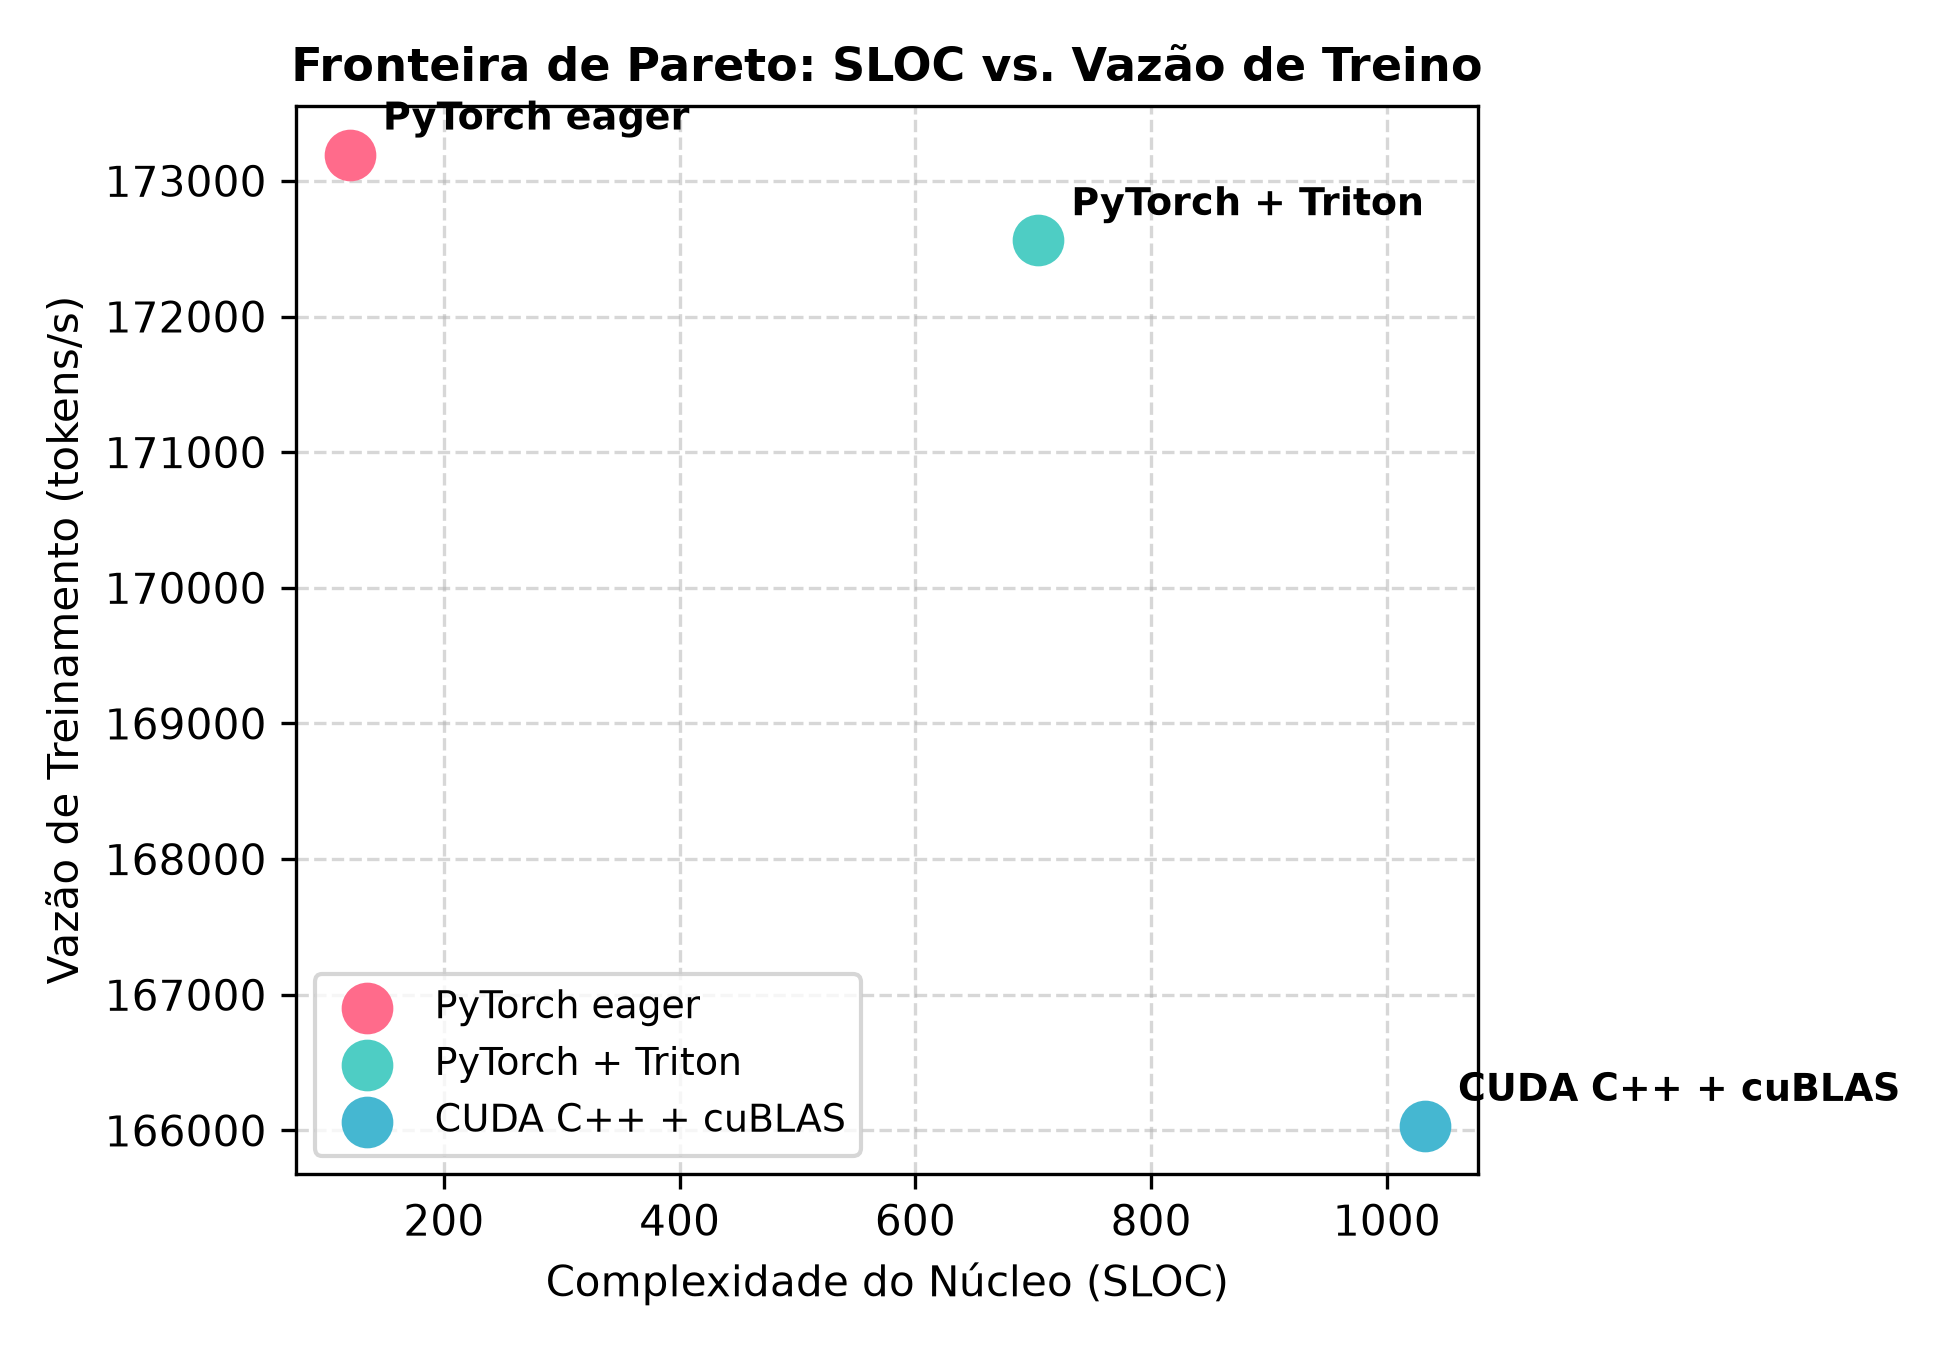
\includegraphics[width=0.8\columnwidth]{pareto_sloc_vs_throughput.png}
\caption{SLOC do núcleo contra vazão de treinamento. O PyTorch ocupa sozinho a fronteira de Pareto nesse regime.}
\label{fig:pareto}
\end{figure}

\subsection{Ameaças à Validade}

Quatro limitações restringem a generalização dos resultados. Primeiro, cada configuração foi executada uma única vez, sem intervalos de confiança. As diferenças de 7\% a 95\% na inferência são grandes em relação à variação típica entre execuções em GPU dedicada, mas a diferença de 0,36\% no treinamento entre PyTorch e Triton deve ser tratada como empate. Segundo, o experimento usa FP32 estrito por exigência de paridade. Com TF32 ou BF16, as GEMMs seriam aceleradas pelos Tensor Cores e a fração de tempo limitada por memória cresceria, o que tende a favorecer a fusão de operadores. Terceiro, a geração não usa KV-\textit{cache}, o que aumenta o trabalho por token em relação a sistemas de produção. Quarto, as atribuições de custo de despacho na inferência com lote 1 são inferências a partir dos tempos totais e não medições de perfilador.

% ======================================================================
\section{Conclusão}
\label{sec:conclusao}

Este trabalho mediu o efeito do nível de abstração de programação em GPU sobre o treinamento e a inferência de um Transformer de 10,8~milhões de parâmetros, com três implementações numericamente equivalentes executadas em FP32 estrito na mesma A100. A equivalência foi verificada no passo inicial, com perda idêntica de 4,175149, e ao longo de 5.000 passos, com perda final de treino de aproximadamente 0,192 nas três versões. Essa verificação permite atribuir as diferenças de desempenho exclusivamente à implementação.

A resposta à questão de pesquisa é que o nível de abstração mais adequado depende do gargalo dominante em cada regime. Na geração com lote 1, o gargalo é o despacho na CPU, e o CUDA C++ reduz a latência para 2,00~ms por token, contra 3,90~ms no PyTorch. Com lote 64, o gargalo passa a ser o tráfego da matriz de atenção na HBM, e o FlashAttention em Triton alcança a maior vazão, 2.716,9~tokens/s, além de reduzir o pico de memória de treino em 16,3\%. No treinamento em FP32, as GEMMs no cuBLAS dominam o tempo de cada passo, e as 120 linhas do PyTorch entregam a mesma vazão que as 704 linhas do Triton e 4\% mais que as 1.032 linhas do CUDA C++.

Na prática, os resultados indicam uma ordem de adoção. O PyTorch \textit{eager} deve ser o ponto de partida para o treinamento. Kernels Triton são justificados quando a carga é limitada por memória, como na atenção com lotes e contextos grandes. Um motor nativo se justifica quando a latência de requisições individuais é o requisito principal. O estudo se limita a um modelo pequeno, a uma única GPU, a FP32 e a execuções únicas. Como trabalhos futuros, propomos repetir as medições com múltiplas sementes de execução, avaliar precisões mistas com Tensor Cores, incluir KV-\textit{cache} e captura de grafos CUDA, que reduz o custo de despacho sem abandonar o PyTorch, e comparar o compilador \texttt{torch.compile}~\cite{ansel2024pytorch2}, que gera kernels Triton automaticamente, com os kernels escritos à mão.

% ======================================================================
\begin{thebibliography}{99}
\bibitem{vaswani2017attention}
A. Vaswani \textit{et al.}, ``Attention is all you need,'' in \textit{Advances in Neural Information Processing Systems (NeurIPS)}, vol. 30, 2017.

\bibitem{radford2019language}
A. Radford \textit{et al.}, ``Language models are unsupervised multitask learners,'' \textit{OpenAI Blog}, vol. 1, no. 8, p. 9, 2019.

\bibitem{paszke2019pytorch}
A. Paszke \textit{et al.}, ``PyTorch: An imperative style, high-performance deep learning library,'' in \textit{Advances in Neural Information Processing Systems (NeurIPS)}, vol. 32, 2019.

\bibitem{ivanov2021data}
A. Ivanov, N. Dryden, T. Ben-Nun, S. Li, and T. Hoefler, ``Data movement is all you need: A case study on optimizing transformers,'' in \textit{Proc. Machine Learning and Systems (MLSys)}, vol. 3, 2021, pp. 711--732.

\bibitem{tillet2019triton}
P. Tillet, H.-T. Kung, and D. Cox, ``Triton: An intermediate language and compiler for tiled neural network computations,'' in \textit{Proc. 3rd ACM SIGPLAN International Workshop on Machine Learning and Programming Languages (MAPL)}, 2019, pp. 10--19.

\bibitem{karpathy2024llmc}
A. Karpathy, ``llm.c: LLM training in simple, raw C/CUDA,'' GitHub repository, 2024. [Online]. Available: \url{https://github.com/karpathy/llm.c}

\bibitem{dao2022flashattention}
T. Dao, D. Y. Fu, S. Ermon, A. Rudra, and C. R{\'e}, ``FlashAttention: Fast and memory-efficient exact attention with IO-awareness,'' in \textit{Advances in Neural Information Processing Systems (NeurIPS)}, vol. 35, 2022, pp. 16344--16359.

\bibitem{xiong2020layer}
R. Xiong \textit{et al.}, ``On layer normalization in the transformer architecture,'' in \textit{Proc. 37th International Conference on Machine Learning (ICML)}, 2020, pp. 10524--10533.

\bibitem{nvidia2020a100}
NVIDIA Corporation, ``NVIDIA A100 Tensor Core GPU architecture,'' White paper, 2020.

\bibitem{williams2009roofline}
S. Williams, A. Waterman, and D. Patterson, ``Roofline: An insightful visual performance model for multicore architectures,'' \textit{Communications of the ACM}, vol. 52, no. 4, pp. 65--76, 2009.

\bibitem{dao2024flashattention2}
T. Dao, ``FlashAttention-2: Faster attention with better parallelism and work partitioning,'' in \textit{International Conference on Learning Representations (ICLR)}, 2024.

\bibitem{milakov2018online}
M. Milakov and N. Gimelshein, ``Online normalizer calculation for softmax,'' \textit{arXiv preprint arXiv:1805.02867}, 2018.

\bibitem{loshchilov2019decoupled}
I. Loshchilov and F. Hutter, ``Decoupled weight decay regularization,'' in \textit{International Conference on Learning Representations (ICLR)}, 2019.

\bibitem{karpathy2023nanogpt}
A. Karpathy, ``ng-video-lecture: Building a GPT from scratch,'' GitHub repository, 2023. [Online]. Available: \url{https://github.com/karpathy/ng-video-lecture}

\bibitem{goldberg1991floating}
D. Goldberg, ``What every computer scientist should know about floating-point arithmetic,'' \textit{ACM Computing Surveys}, vol. 23, no. 1, pp. 5--48, 1991.

\bibitem{ansel2024pytorch2}
J. Ansel \textit{et al.}, ``PyTorch 2: Faster machine learning through dynamic Python bytecode transformation and graph compilation,'' in \textit{Proc. 29th ACM International Conference on Architectural Support for Programming Languages and Operating Systems (ASPLOS)}, 2024, pp. 929--947.
\end{thebibliography}

\end{document}
